\section{Parametric sensitivity analysis}\label{sec:sensitivity_study}
\noindent This section performs a parametric sensitivity study on the reference tracking performance of \ac{DeePC}, \ac{CL-DeePC}, and the oracle, thereby providing contribution~5. Investigated parameters are the number of past data points $\bar{N}$, the innovation noise variance $\Sigma(e_k)$, and the window lengths $p=f$. As a measure of the reference tracking performance the root mean square of the reference tracking error, scaled by the root mean square of the reference signal, is used. To reflect purely the effect on performance during adaptive closed-loop operation, the presented means exclude the first $\bar{N}$ control actions, which rely in part on open-loop data. Note that in general it is theoretically possible for \ac{DeePC} and \ac{CL-DeePC} to outperform the employed oracle because the oracle does (also) not account for noise.

\subsection{Number of past data samples: $\bar{N}$}
\noindent The effect of a varying number of past data samples $\bar{N}$ is shown in Fig.~\ref{fig:varying_Nbar}. Slight undulations of the displayed oracle performance are an artifact that is attributable to averaging over the last $1800-\bar{N}$ samples of a simulation to exclude control actions that are based on open-loop data. Using \ac{CL-DeePC} the reference tracking performance approaches the oracle's performance at a relatively low $\bar{N}$. For \ac{DeePC} the picture is different, with the median reference tracking performance remaining $26\%$ higher than its oracle counterpart at $\bar{N}=1039$. By comparison this value is only $4\%$ for \ac{CL-DeePC}.

Fig.~\ref{fig:varying_Nbar} demonstrates that \ac{CL-DeePC} is what we refer to as more `sample efficient' than \ac{DeePC}; in general \ac{CL-DeePC} is able to use fewer past data samples to obtain as good or better performance. The improved sample efficiency of \ac{CL-DeePC} is attributable to the fact that a shorter future prediction window length is implicitly used for identification by \ac{CL-DeePC} when compared to \ac{DeePC} ($f_\mathrm{ID}=1$ as opposed to $f_\mathrm{ID}=f$). This leaves more columns $N=\bar{N}-p-f_\mathrm{ID}+1$ to approximate the relevant correlation matrices that are used implicitly by both \ac{DeePC} and \ac{CL-DeePC} (consider, for instance, $\hat{\Sigma}_{yz}$, $\hat{\Sigma}_{\psi z}$ from~\eqref{eq:Yfhat_1}). In addition, the discussed closed-loop identification issue entails that even if $\bar{N}$ (and therefore $N$) is large such that these correlation matrices are approximated well, \ac{DeePC} still performs worse than \ac{CL-DeePC}.
% ------------------------- Figure --------------------------
\begin{figure}[t!]
\begin{center}
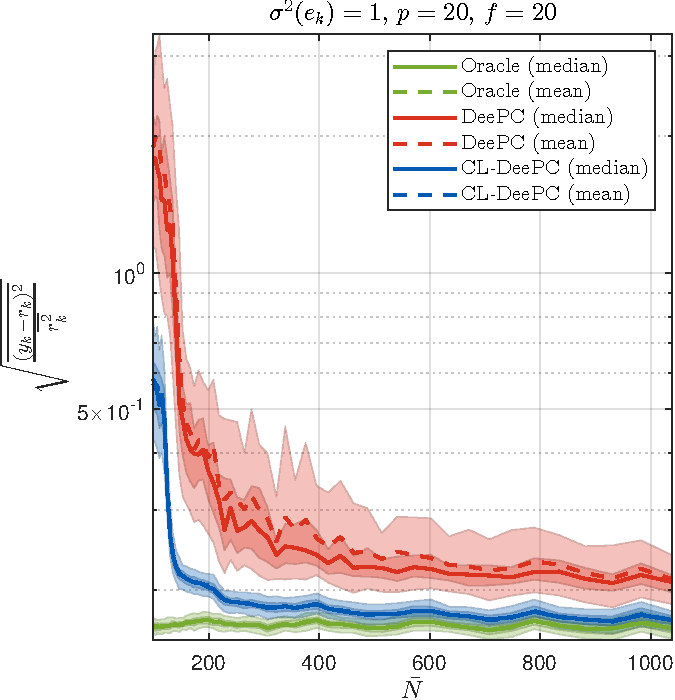
\includegraphics[width=\columnwidth]{results/figures/Varying_Nbar_99-1039-50_p_20_f_20_Re_1_Ru_1_Rdu_0_Q_100_R_0_dR_10.pdf}    % The printed column  
\caption{Effect of varying $\bar{N}$ on reference tracking performance. Shaded regions indicate the 1st, 3rd, 7th and 9th deciles of 120 simulations with different noise realizations.}  % width is 8.4 cm.
\label{fig:varying_Nbar}                                 % Size the figures 
\end{center}                                 % accordingly.
\end{figure}
% -----------------------------------------------------------

\subsection{Noise level: $\Sigma(e_k)$}
\noindent The effect of the noise level, as quantified by a varying innovation noise variance $\Sigma(e_k)$, is shown in Fig.~\ref{fig:varying_Re}. In the absence of noise, \ac{DeePC} and \ac{MPC} are equivalent~\cite{Coulson2019}, and the aforementioned closed-loop identification issue does not exist. Hence, as demonstrated by the figure, the reference tracking performance of the three algorithms is identical in the noiseless case. As the noise level increases, correlation between inputs and preceding noise increases because $|e_k|$ is typically larger, and more control effort is needed to perform noise rejection. Consequently, the closed-loop identification issue becomes more troublesome for \ac{DeePC} at higher noise levels. Note that the performance of all methods decreases with an increasing noise level because all methods lack the ability to immediately compensate noise disturbances. The mean slopes of the median reference tracking performance over the complete range of shown noise levels are 0.0762, 0.0958, and 0.1848 for respectively the oracle, \ac{CL-DeePC}, and \ac{DeePC}. Using this as a measure for the susceptibility to noise, these slopes indicate that, e.g., the reference tracking performance of \ac{CL-DeePC} is 48\% less susceptible to noise-induced deterioration compared to \ac{DeePC}.
% ------------------------- Figure --------------------------
\begin{figure}[t!]
\begin{center}
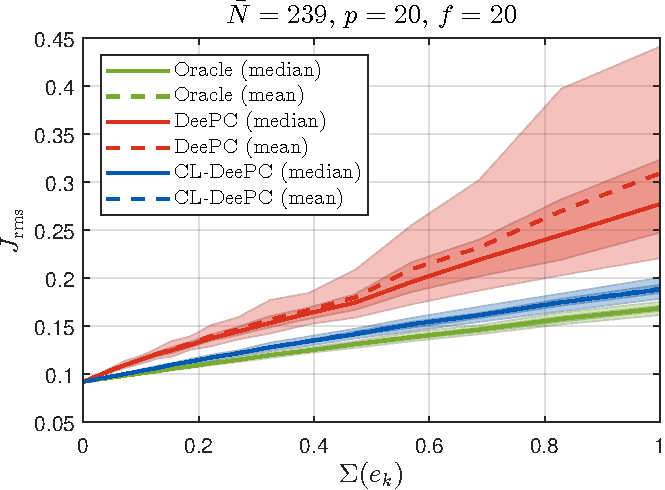
\includegraphics[width=\columnwidth]{results/figures/Varying_Re_0.0001-1-50_Nbar_239_p_20_f_20_Ru_1_Rdu_0_Q_100_R_0_dR_10.pdf}    % The printed column 
\caption{Effect of varying $\Sigma(e_k)$ on reference tracking performance. Shaded regions indicate the 1st, 3rd, 7th and 9th deciles of 120 simulations with different noise realizations.}  % width is 8.4 cm.
\label{fig:varying_Re}                                 % Size the figures 
\end{center}                                 % accordingly.
\end{figure}
% -----------------------------------------------------------

\subsection{Past data window lengths: $p=f$}
\noindent For the sake of simplicity, and the fact that $p=f$ is a typical choice in the closely related field of subspace identification~\citep{vanderVeen2013}, this is also the choice made in this work. We discern two competing mechanisms to explain the results shown in Fig.~\ref{fig:varying_pf} for \ac{CL-DeePC} and an additional detrimental effect on performance for \ac{DeePC}. Increasing $p$ is beneficial in terms of reducing the bias of the predictor. However, as with increasing $f_\mathrm{ID}$, increasing $p$ entails implicitly estimating more parameters of the predictor, thereby increasing its variance. This is more pronounced for \ac{DeePC} since $f_\mathrm{ID}=f$ when compared to \ac{CL-DeePC} for which $f_\mathrm{ID}=1$. The shorter future window length used for identification $f_\mathrm{ID}$ is also beneficial for \ac{CL-DeePC} because a higher degree of collinearity may be expected for larger $f_\mathrm{ID}$, potentially leading to ill conditioning of the identification task~\citep{Chiuso2004}. Together with the aforementioned closed-loop identification issue these effects induce up to a 49\% lower reference tracking cost at $p=f=100$ for \ac{CL-DeePC} compared to \ac{DeePC}. Moreover, note that the performance of \ac{DeePC} deteriorates rapidly with increasing $p=f$, whilst the impact on the performance of \ac{CL-DeePC} is far less pronounced.
% 1) period of 200 time samples\\
% 2) increase p -> smaller bias, but larger variance (increase number of estimated parameters)\\
% 3) increasing collinearity \& ill conditioning\\
% ------------------------- Figure --------------------------
\begin{figure}[t!]
\begin{center}
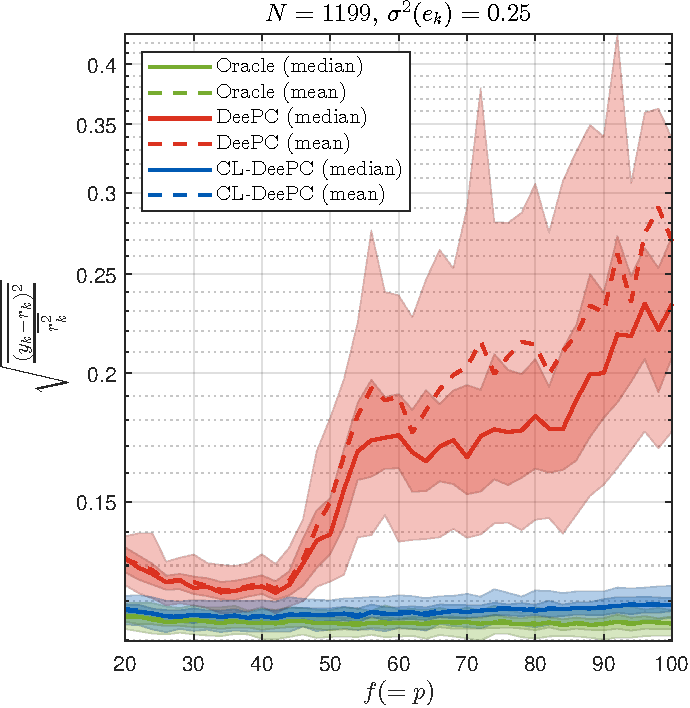
\includegraphics[width=\columnwidth]{results/figures/Varying_pf_20-100-41_Nbar_1199_Re_0.25_Ru_1_Rdu_0_Q_100_R_0_dR_10.pdf}    % The printed column 
\caption{Effect of varying $f=p$ on reference tracking performance. Shaded regions indicate the 1st, 3rd, 7th and 9th deciles of 120 simulations with different noise realizations.}  % width is 8.4 cm.
\label{fig:varying_pf}                                 % Size the figures 
\end{center}                                 % accordingly.
\end{figure}
% -----------------------------------------------------------
